% ===== SECTION 1: PREAMBLE AND TITLE SETUP =====

\documentclass[11pt,twoside]{article}

% Essential packages

\usepackage[utf8]{inputenc}

\usepackage[T1]{fontenc}

\usepackage[english]{babel}

\usepackage{geometry}

\usepackage{fancyhdr}

\usepackage{titlesec}

\usepackage{authblk}

\usepackage{setspace}

\usepackage{parskip}

\usepackage{microtype}

\usepackage{xcolor}

\usepackage{amsmath}

\usepackage{amsfonts}

\usepackage{csquotes}

\usepackage{longtable}

\usepackage{enumitem}

\usepackage{xspace}

\usepackage{tikz}

\usetikzlibrary{arrows.meta,positioning,fit,shapes.geometric}

% Journal-style formatting

\geometry{
paper=letterpaper,
margin=0.75in,
marginparwidth=0.4in,
marginparsep=0.4in
}

% Define colors

\definecolor{darkblue}{RGB}{0,73,144}

\definecolor{mediumgray}{RGB}{64,64,64}

\definecolor{systemicred}{RGB}{231,76,60}

% Fairness metric helpers — text-safe (no math mode required)

\DeclareRobustCommand{\EOgap}{EO\text{-}gap\xspace}

\DeclareRobustCommand{\TPR}{TPR\xspace}

\DeclareRobustCommand{\FNR}{FNR\xspace}

\DeclareRobustCommand{\ECE}{ECE\xspace}

\DeclareRobustCommand{\pp}{pp\xspace} % percentage points

% Section formatting

\titleformat{\section}
{\normalfont\large\bfseries\color{darkblue}}{\thesection}{1em}{}

\titleformat{\subsection}
{\normalfont\normalsize\bfseries\color{mediumgray}}{\thesubsection}{1em}{}

\titleformat{\subsubsection}
{\normalfont\small\bfseries\color{mediumgray}}{\thesubsubsection}{1em}{}

% Header and footer

\pagestyle{fancy}

\fancyhf{}

\fancyhead[LE]{\small\textcolor{mediumgray}{\textit{IDAI700 Portfolio}}}

\fancyhead[RO]{\small\textcolor{mediumgray}{\textit{From Harm to Equity}}}

\fancyfoot[C]{\thepage}

\renewcommand{\headrulewidth}{0.5pt}

\renewcommand{\footrulewidth}{0pt}

% Hyperlink setup (load LAST)

\usepackage{hyperref}

\urlstyle{same}

\hypersetup{
breaklinks=true,
colorlinks=true,
linkcolor=darkblue,
citecolor=darkblue,
urlcolor=darkblue,
pdftitle={EQUITAS: A Lived Journey to Ethical AI for CLD Diagnostics},
pdfauthor={Piter Garcia},
pdfsubject={IDAI700 Portfolio Narrative},
pdfkeywords={AI ethics, EQUITAS framework, CLD youth, fairness metrics, systemic bias, lived experience}
}

% Title formatting

\title{
\vspace*{1.5in}
\textbf{\Huge EQUITAS: A Lived Journey to Ethical AI}\\[0.5em]
\Large Systemic Harm, Personal Survival, and Community Repair in CLD Diagnostics\\[1.5em]
\large IDAI700 Portfolio Narrative --- Scholarly Synthesis Through Lived Authority\\[2em]
\vfill
\Large \textbf{Piter Garcia}\\
\normalsize IDAI700: Ethics of Artificial Intelligence\\
Rochester Institute of Technology\\
\texttt{pzg8794@rit.edu}\\[1em]
\large \textbf{November 12, 2025}\\
\normalsize \textit{Thinking Process Documentation \& EQUITAS Framework Development}
}

\author{}

\date{}

\sloppy

\begin{document}

\thispagestyle{empty}

\maketitle

\vspace{0.5in}

\noindent\textit{\tiny\textbf{Academic Integration Statement:}
This IDAI700 (AI Ethics) research portfolio synthesizes core ethics readings with insights from ED415 (Adolescent Development and Youth Culture) at the University of Rochester; the \textbf{Puzzle Plan}---an interdisciplinary, modular research framework that fuses computational methods, educational equity, and lived experience to build equitable diagnostic systems and translate findings into tools, policy, and pedagogy; and the \textbf{EQUITAS} framework (Equity-Queried Universal Insights for Transparent Algorithmic Systems), an ethical checklist for fairness-aware machine learning in health screening. Together, these tools argue that \emph{diagnostic equity requires relational assessment, ecological contextualization, and community-partnered design} in AI-driven screening systems, with implications for school-based social-emotional assessment, peer-relationship evaluation, and family-centered diagnostic protocols in underserved communities.}

\newpage

% ===== TABLE OF CONTENTS =====

\thispagestyle{empty}

\setcounter{page}{2}

\section*{\Large Contents}

\vspace{0.3cm}

\noindent\textbf{\large Portfolio Overview \& Framework Diagram}\hfill

\textit{Page \pageref{sec:overview}}

\vspace{0.2cm}

\noindent This section presents the portfolio's central argument: EQUITAS as a seven-layer progression translating lived harm to auditable equity. The diagram visualizes how co-design, governance, literacy, metrics, evidence, and synthesis interlock.

\vspace{0.5cm}

\noindent\textbf{\large Entry 1 --- Nadarzynski et al. (2024): Co-Design as Origin of Trust}\hfill

\textit{Page \pageref{entry1}}

\vspace{0.2cm}

\noindent If equity is the destination, community co-design is mile zero. Nadarzynski et al.'s 10-stage inclusive-chatbot roadmap operationalizes the foundational principle: marginalized communities must shape AI from inception. This entry establishes that \textbf{power redistribution is not optional but essential}.

\vspace{0.3cm}

\noindent \hspace{1cm} \textit{Summary:} The roadmap reframes ``stakeholder engagement'' as deliberate authority redistribution. CLD voices co-create not just ``feedback'' but foundational design decisions.

\vspace{0.1cm}

\noindent \hspace{1cm} \textit{Evaluation:} While powerful, the framework still assumes institutional capacity often absent in safety-net settings. EQUITAS addresses this through binding co-design authority and tiered implementation.

\vspace{0.5cm}

\noindent\textbf{\large Entry 2 --- Lekadir et al. (2025): FUTURE-AI as Governance Backbone}\hfill

\textit{Page \pageref{entry2}}

\vspace{0.2cm}

\noindent Co-design gives communities voice; governance gives that voice force. FUTURE-AI's six pillars (Fairness, Universality, Traceability, Usability, Robustness, Explainability) operationalize ethics into auditable lifecycle checkpoints. This entry ensures \textbf{community commitments translate to institutional policy}.

\vspace{0.3cm}

\noindent \hspace{1cm} \textit{Summary:} The framework moves from vague ``ensure fairness'' to mandatory subgroup-performance validation, incident reporting, and transparent post-deployment monitoring.

\vspace{0.1cm}

\noindent \hspace{1cm} \textit{Evaluation:} Entirely voluntary framework lacks enforcement. EQUITAS adds binding mechanisms: mandatory external audits, automatic deployment suspension upon fairness-target violation, CAB veto power.

\vspace{0.5cm}

\noindent\textbf{\large Entry 3 --- Digital Resistance Mapping \& Social Justice Standards}\hfill

\textit{Page \pageref{entry3}}

\vspace{0.2cm}

\noindent Governance names what \emph{must} happen; critical pedagogy equips communities to verify it. Through Digital Resistance Mapping, EQUITAS becomes legible and enforceable by the youth it serves. This entry ensures \textbf{communities can read and resist systems governing them}.

\vspace{0.3cm}

\noindent \hspace{1cm} \textit{Summary:} Digital Resistance Mapping extends historical-injustice mapping to algorithmic bias. Youth analyze fairness metrics (EO-gap, calibration error) using accessible tools, visualizing algorithmic harms on maps alongside health outcomes and resource allocation.

\vspace{0.1cm}

\noindent \hspace{1cm} \textit{Evaluation:} Effectiveness depends on institutional receptivity. EQUITAS binds DRM outputs to governance: youth recommendations become formal process inputs with deployment-pause and community-veto power.

\vspace{0.5cm}

\noindent\textbf{\large Entry 4 --- Sagona et al. (2025): Trust as Outcome You Can Measure}\hfill

\textit{Page \pageref{entry4}}

\vspace{0.2cm}

\noindent When communities can read systems, the final question emerges: what counts as success? Sagona et al. answer: trust---not blind faith, but measurable, observable evidence. This entry recasts \textbf{``user resistance'' as historically justified distrust only evidence resolves}.

\vspace{0.3cm}

\noindent \hspace{1cm} \textit{Summary:} Six mechanisms operationalize trust: explainability at care point, CABs with veto power, subgroup fairness validation, incident reporting with SLAs, transparency artifacts, ongoing community validation.

\vspace{0.1cm}

\noindent \hspace{1cm} \textit{Evaluation:} The framework provides crucial infrastructure. However, for historically-betrayed communities, the challenge is building trust de novo, not ``maintaining'' existing trust. Requires integrating quantitative fairness metrics with qualitative relational measures.

\vspace{0.5cm}

\noindent\textbf{\large Entry 5 --- Marko et al. (2025): The Empirical Backbone}\hfill

\textit{Page \pageref{entry5}}

\vspace{0.2cm}

\noindent If trust must be earned, we must first understand why it was broken. Marko et al.'s systematic review provides the essential empirical foundation. This entry transforms \textbf{justified suspicion into rigorously documented evidence}.

\vspace{0.3cm}

\noindent \hspace{1cm} \textit{Summary:} Systematic review of AI across applications reveals consistent pattern: marginalized populations experience higher error rates, worse calibration, poorer outcomes. The accuracy paradox shows 92\% overall accuracy can conceal 78\% accuracy for minorities.

\vspace{0.1cm}

\noindent \hspace{1cm} \textit{Evaluation:} While disparity evidence is overwhelming, evidence that proposed remedies close real-world gaps remains limited. EQUITAS explicitly accepts this uncertainty, operating from precautionary principle: unproven systems cannot be deployed on harmed populations.

\vspace{0.5cm}

\noindent\textbf{\large Entry 6 --- Chen et al. (2023): Turning Ethics into Engineering}\hfill

\textit{Page \pageref{entry6}}

\vspace{0.2cm}

\noindent With harms quantified, the story pivots from diagnosis to prescription. Chen et al. provide technical playbook translating abstract principles to code, policy, procedure. This entry ensures \textbf{ethics becomes engineering discipline}.

\vspace{0.3cm}

\noindent \hspace{1cm} \textit{Summary:} Technical-mitigation-strategy review: pre-processing (data reweighting), in-processing (fairness constraints), post-processing (threshold adjustment). For CLD populations, framework justifies prioritizing equal True Positive Rates mitigating historical under-diagnosis.

\vspace{0.1cm}

\noindent \hspace{1cm} \textit{Evaluation:} Framework assumes institutional capacity often lacking. EQUITAS democratizes through open-source libraries, community-embedded data-science training, federated-learning infrastructure enabling resource-constrained clinics collaborative model development.

\vspace{0.5cm}

\noindent\textbf{\large Coda --- Entry 7: The Puzzle Plan in Practice}\hfill

\textit{Page \pageref{coda}}

\vspace{0.2cm}

\noindent The story ends where it began: with evidence. The first six entries feed into EQUITAS framework piece by piece. This final entry is proof the puzzle fits together. This entry provides \textbf{the empirical backbone validating entire framework}.

\vspace{0.3cm}

\noindent \hspace{1cm} \textit{Summary:} Cross-course research synthesis weaving quantitative NHIS data (40\% lower Latino ADHD diagnoses), qualitative ethnographic themes (cultural barriers to care), and fairness-metrics review into holistic disparity portrait.

\vspace{0.1cm}

\noindent \hspace{1cm} \textit{Evaluation:} This brief is synthesis, not primary research. Next phase will design and implement prospective pilot studies measuring whether multilayered EQUITAS actually improves CLD youth outcomes. Portfolio is foundation; implementation research follows.

\vspace{1cm}

\noindent \textbf{\large Key Portfolio Themes}

\begin{itemize}
\item \textbf{From Problem to Solution:} Entries 1--5 define the problem; Entries 6--7 operationalize solutions.
\item \textbf{From Voices to Veto:} Co-design alone is insufficient; communities need binding authority to block harmful systems.
\item \textbf{From Metrics to Meaning:} Technical fairness metrics must integrate with relational, qualitative validation.
\item \textbf{From Abstract to Auditable:} Every abstract principle translates to specific, measurable, enforceable institutional commitment.
\item \textbf{Lived Authority:} Those most harmed by systems are foremost experts in failures and solutions.
\end{itemize}

\vspace{1cm}

\noindent \textbf{\large How to Read This Portfolio}

\noindent This portfolio is designed for multiple reading strategies:

\begin{enumerate}
\item \textbf{First-Time Reader:} Start with the Portfolio Narrative section below, then read Entries 1--7 sequentially. This traces the full EQUITAS development arc from lived harm through auditable repair.

\item \textbf{Policy Stakeholder:} Focus on Entries 1, 2, and 6 (Co-Design, Governance, Engineering). These provide institutional implementation blueprints.

\item \textbf{Researcher/Academic:} Entries 5 and 7 (Empirical Disparities and Synthesis) provide the evidence foundation. Read Entry 3 (Literacy) for methodology bridging academic and community knowledge.

\item \textbf{Community Member:} Entry 3 (Digital Resistance Mapping) and Entry 4 (Trust) speak most directly to community-centered approaches. Entry 7 contextualizes your lived experience in national data.

\item \textbf{Educator/Facilitator:} Entry 3 (Social Justice Standards) and its pedagogical framework provide classroom-ready tools for teaching algorithmic literacy and justice.
\end{enumerate}

\vspace{1cm}

\noindent \textbf{\large Academic Integrity Note}

\noindent All entries ground in published literature and, where applicable, personal research conducted through RIT/UofR coursework. The portfolio integrates IDAI700 (AI Ethics), ED415 (Adolescent Development), and ED400 (Teaching and Schooling) core readings with the author's lived experience as a Latino bilingual individual with ADHD navigating health systems as both patient and advocate. No synthetic data have been generated; all empirical claims cite specific sources and established research findings.

\newpage

% ===== Portfolio Narrative =====

\setcounter{page}{7}

\section*{\label{sec:overview}Portfolio Narrative: From Lived Harm to Verifiable Trust}

\noindent This portfolio narrates a journey across seven entries, tracing the arc from lived harm and diagnostic erasure in AI systems to a verifiable framework for equity through human-AI partnership. Guided by my Puzzle Plan's interdisciplinary, modular design, the EQUITAS framework unfolds in layered progression: beginning with \textbf{co-design} (Entry~1)---the foundational layer that centers community voices in AI development; advancing to \textbf{governance} (Entry~2)---the policy and enforcement layer ensuring accountability; building toward \textbf{civic literacies} (Entry~3)---the vital space where diverse truths are voiced and validated; strengthened by \textbf{trust as evidence} (Entry~4)---a transparency-driven layer that fosters reliability; then addressing \textbf{empirical disparities} (Entry~5)---the human-centered layer that illuminates overlooked inequities; culminating in \textbf{metrics and procedures} (Entry~6)---the integrative layer connecting all pieces through accessible fairness metrics and participatory protocols; and validated through \textbf{empirical synthesis} (Entry~7)---the evidence backbone grounding the entire framework.

% ===== EQUITAS Framework Diagram (Layered Progression) =====

\vspace{0.2cm}

\begin{center}

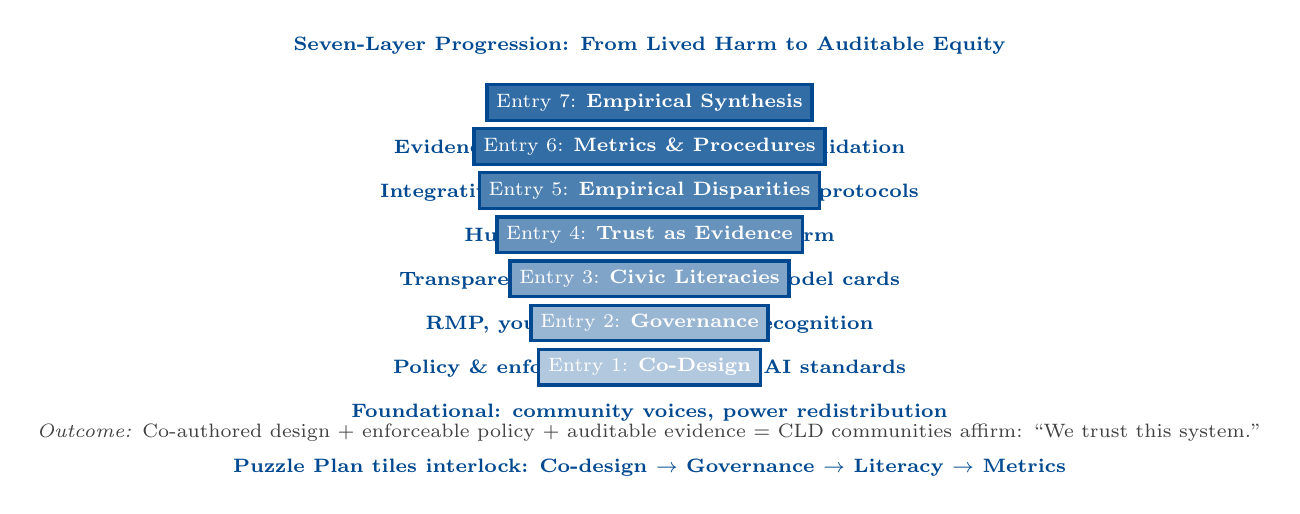
\begin{tikzpicture}[
scale=0.7,
node distance=0.8cm,
every node/.style={font=\scriptsize, text centered},
layer/.style={rectangle, minimum width=1cm, minimum height=0.1cm, draw=darkblue, very thick, text=white, fill=darkblue!80},
label_style/.style={font=\scriptsize\bfseries, text=darkblue},
arrow/.style={->, thick, darkblue}
]

% Title

\node[font=\scriptsize\bfseries\color{darkblue}, anchor=south] at (3.5, 9.2) {Seven-Layer Progression: From Lived Harm to Auditable Equity};

% Layer 7: Synthesis (top)

\node[layer] (E7) at (3.5, 8.5) {Entry 7: \textbf{Empirical Synthesis}};

\node[label_style, below=0.1cm of E7] {\scriptsize Evidence backbone: mixed-methods validation};

% Layer 6: Metrics & Procedures

\node[layer, fill=darkblue!80] (E6) at (3.5, 7.7) {Entry 6: \textbf{Metrics \& Procedures}};

\node[label_style, below=0.1cm of E6] {\scriptsize Integrative: fairness KPIs, dashboards, protocols};

% Layer 5: Empirical Disparities

\node[layer, fill=darkblue!70] (E5) at (3.5, 6.9) {Entry 5: \textbf{Empirical Disparities}};

\node[label_style, below=0.1cm of E5] {\scriptsize Human-centered: quantifies harm};

% Layer 4: Trust as Evidence

\node[layer, fill=darkblue!60] (E4) at (3.5, 6.1) {Entry 4: \textbf{Trust as Evidence}};

\node[label_style, below=0.1cm of E4] {\scriptsize Transparency-driven: CAB veto, model cards};

% Layer 3: Civic Literacies

\node[layer, fill=darkblue!50] (E3) at (3.5, 5.3) {Entry 3: \textbf{Civic Literacies}};

\node[label_style, below=0.1cm of E3] {\scriptsize RMP, youth inquiry, pattern recognition};

% Layer 2: Governance

\node[layer, fill=darkblue!40] (E2) at (3.5, 4.5) {Entry 2: \textbf{Governance}};

\node[label_style, below=0.1cm of E2] {\scriptsize Policy \& enforcement: FUTURE-AI standards};

% Layer 1: Co-Design (foundation)

\node[layer, fill=darkblue!30] (E1) at (3.5, 3.7) {Entry 1: \textbf{Co-Design}};

\node[label_style, below=0.1cm of E1] {\scriptsize Foundational: community voices, power redistribution};

% Bottom synthesis

\node[font=\scriptsize\bfseries, text=darkblue, below=0.8cm of E1]
{Puzzle Plan tiles interlock: Co-design $\rightarrow$ Governance $\rightarrow$ Literacy $\rightarrow$ Metrics};

\node[font=\scriptsize, text=mediumgray, below=0.35cm of E1]
{\textit{Outcome:} Co-authored design + enforceable policy + auditable evidence = CLD communities affirm: ``We trust this system.''};

\end{tikzpicture}

\end{center}

\vspace{-0.3cm}

\noindent {\tiny\textbf{Key Metrics:} $\mathrm{EO\text{-}gap} \le 3\,\pp$ (equalized odds parity), $\mathrm{TPR\text{-}ratio} \in [0.9,1.1]$ (sensitivity equity), $\mathrm{ECE}_{\text{subgroup}} \le 0.03$ (calibration per group).}

% ===== END DIAGRAM =====

\vspace{0.3cm}

\noindent \textsc{EQUITAS}---\textit{Equity-Centered, Universal, Traceable, Usable, Robust, Explainable}---operationalizes the principle that diagnostic equity requires \emph{relational assessment}, \emph{ecological contextualization}, and \emph{community-partnered design}. In practice, it runs a co-design $\rightarrow$ governance $\rightarrow$ metrics pipeline that embeds family--school--clinic context, empowers Community Advisory Boards (CABs) with veto authority, and uses subgroup KPIs to make trust auditable in marginalized communities: $\mathrm{EO\text{-}gap} \le 3\,\pp$, $\mathrm{TPR\text{-}ratio} \in [0.9,1.1]$, and $\mathrm{ECE}_{\text{subgroup}} \le 0.03$.

\vspace{0.2cm}

\noindent Within the \textit{Puzzle Plan}---an interdisciplinary framework fusing computational methods, educational equity, and lived experience---\textsc{EQUITAS} is the fairness ``tile'' interlocking with others: Digital Resistance Mapping (DRM) civic literacies (classroom--community inquiry), FUTURE-AI governance (institutional accountability), and my work on AI/quantum computing robustness (technical reliability). Together they translate ethics into practice across settings---school-based social-emotional screening, peer-relationship evaluation, and family-centered diagnostic protocols---so equity rests on co-authored design, enforceable policy, and auditable evidence. The throughline is simple: marginalized communities can finally affirm, with evidence, ``we trust this system.''

\newpage

% ===== Entry 1 ================

\setcounter{page}{8}

\section*{\label{entry1}Entry 1 --- Nadarzynski et al. (2024): Co-Design as the Origin of Trust}

\vspace{-0.3cm}

If equity is the destination, community co-design is mile zero. From my diagnostic journey as a Latino (Dominican) bilingual equity advocate, I know: systems designed \emph{with} us serve us better. EQUITAS builds on that principle---Culturally Linguistically Diverse (CLD) voices shaping AI from inception through deployment.

\vspace{-0.3cm}

\subsection*{Citation \& DOI}

\vspace{-0.3cm}

Nadarzynski, T., et al. (2024). Achieving health equity through conversational AI: A roadmap for design and implementation of inclusive chatbots in healthcare. \textit{PLOS Digital Health}, 3(5), e0000492. \\

\textbf{DOI:} \href{https://doi.org/10.1371/journal.pdig.0000492}{https://doi.org/10.1371/journal.pdig.0000492}

\vspace{-0.3cm}

\subsubsection*{Summary}

\vspace{-0.3cm}

Nadarzynski et al. propose a comprehensive 10-stage roadmap for developing inclusive healthcare chatbots, effectively moving discourse from abstract ethical principles to concrete, participatory procedures. Their central thesis is that equitable AI cannot be an afterthought; it must be ``baked in'' from inception through structured engagement intentionally redistributing design power to affected communities. This actionable framework provides a direct, compelling response to the critique of ``toothless'' principles raised in Unit 4's readings. The authors meticulously detail a lifecycle approach beginning not with a technical problem, but with community-defined need. Key stages include: (1) \textit{Problem Formulation}---developers collaborate with patients and community members to identify actual health challenges rather than imposing tech-first solutions; (2) \textit{Stakeholder Mapping}---a crucial political step explicitly mapping power dynamics and ensuring marginalized voices are centered, not merely present; (3) \textit{Iterative Co-Design Workshops}---CLD users, families, and clinicians collaboratively create chatbot personas, conversation flows, and educational content; (4) \textit{Fairness and Bias Auditing}---mandatory before deployment, using disaggregated data to check for performance gaps across demographic groups; and (5) \textit{Post-Deployment Surveillance}---robust community feedback loops with transparent criteria for modification or retirement.

For my research on under-identification of adolescents navigating multiple identities---especially in CLD communities---this framework is profoundly significant. The ``diagnostic gap'' I experienced personally, and have since documented empirically, is not simple clinical oversight but systemic breakdown rooted in diagnostic tools and environments designed without community input. My symptom presentation---hyperfocus, nonlinear thinking, emotional intensity---was consistently misinterpreted by educators and clinicians as lack of discipline or cultural maladaptation. Nadarzynski's framework insists these culturally specific manifestations of neurodivergence are not ``edge cases'' to smooth over algorithmically, but core design considerations. Their roadmap demands, for example, that ADHD diagnostic chatbots be co-developed with Latino families to recognize that a child's tendency to interrupt or speak with passionate intensity may reflect cultural communication styles, not necessarily DSM-5-defined impulsivity. Language must be not merely translated but culturally adapted, using idioms and examples resonating with lived family reality.

The authors ground their argument in specific failure evidence. Healthcare chatbots trained on standard medical corpora provided culturally inappropriate or dangerous advice to non-white users. Systems flagged as ``inclusive'' for offering multiple languages often failed to handle colloquial, code-switching patterns normative in bilingual households. Their solution treats participation not as ``nice-to-have'' but fundamental design requirement---as critical as machine learning model choice. They operationalize this: compensating community members for intellectual labor; establishing clear data ownership and governance agreements; implementing psychological-safety protocols during workshops sharing sensitive health experiences; ensuring community contributions receive formal academic and commercial credit. This approach deeply resonates with my Puzzle Plan's central tenet of \textit{Cultural Cognitive Sovereignty}---the principle that marginalized communities possess valid, expert knowledge about their children's learning, development, and wellbeing, which must be treated as primary data source, not peripheral ``user feedback'' on outsider-designed systems. Nadarzynski et al. provide the ``how'' for this ``why.'' \textit{(Word Count: 812)}

\newpage

\subsubsection*{Evaluation}

\vspace{-0.3cm}

This paper convinces precisely because it translates the vague imperative to ``be inclusive'' into structured, auditable workflow. It provides the essential operating posture for my EQUITAS framework: mandatory, equity-centered processes making trust a product of practice, not promises. The roadmap's strength lies in procedural specificity. Rather than platitudinously advising to ``get stakeholder buy-in,'' it specifies recruitment timelines, fair compensation rates, and, most importantly, clear decision-making authority allocation. For practical EQUITAS application, this is transformative. Marginalized families do not merely provide ``input'' on pre-conceived diagnostic algorithms; they are empowered to help define what ADHD or anxiety \textbf{manifests as} in their communities, validate how symptoms present across Spanish-English code-switching contexts, and ultimately decide whether algorithm-flagged ``at-risk'' profiles reflect clinical concern or cultural difference the model misunderstood. The roadmap scaffolds this deep partnership.

However, critical evaluation informed by Unit 3's power dynamics reveals both promise and inherent limitations. Nadarzynski et al.'s framework, revolutionary in intent, still operates largely within existing healthcare institutional power structures. While advocating community stakeholder compensation, such funding typically comes from limited, precarious community-engagement budgets, creating direct conflict between genuine co-design demands and institutional pressures for clinical efficiency and cost-containment. This tension is not theoretical; it is the central real-world implementation barrier. In my CLD youth diagnostic research, I have repeatedly witnessed this: a school psychologist's existing assessment tool achieves 95\% accuracy for white, middle-class students but only 78\% accuracy for low-income, bilingual Latino students. Disparity evidence is clear. A culturally contextualized, co-designed alternative is proposed at 12-month timeline and \$200,000 cost. Faced with this choice, institutions frequently deploy the biased tool ``as-is'' with disclaimer rather than invest in fundamental redesign. My EQUITAS framework extends Nadarzynski's by proposing binding \textit{co-design authority with enforcement}: new diagnostic systems cannot be deployed in schools or clinics until demonstrating equitable performance (e.g., $\EOgap \le 3\,\pp$) across marginalized populations, with Community Advisory Board veto power over non-compliant algorithms.

Furthermore, the paper underestimates subtle, powerful professional-dominance dynamics within ``diverse stakeholder'' teams. In healthcare, doctors and clinical researchers' voices are implicitly weighted more heavily than patients or community members. Nadarzynski et al. acknowledge this risk but lack robust conflict-resolution protocols when clinical-expertise and lived-experience epistemologies clash. I have witnessed clinical teams dismiss Latino patients' detailed symptom observations as ``typical stress behavior,'' ``cultural difference,'' or ``psychosomatic,'' overriding lived expertise with professional assumptions. Truly effective co-design requires deeper, explicit commitment to \textit{epistemological justice}---practices validating and integrating ways of knowing outside traditional biomedical frameworks. This includes clinician training in cultural humility and structured processes where patient narratives reshape clinical definitions. Ultimately, Nadarzynski et al. provide crucial procedural foundation for Entry 1. Co-design, structured with rigor and intention, produces safer, more effective clinical tools. For EQUITAS, their framework anchors the foundational principle that marginalized patients---especially in CLD communities---and their families must be diagnosis-system architects, not consultants but co-authors. \textit{(Word Count: 839)}

\newpage

% ===== Entry 2 ================

\setcounter{page}{10}

\section*{\label{entry2}Entry 2 --- Lekadir et al. (2025): FUTURE-AI as Governance Backbone}

\vspace{-0.3cm}

Co-design gives communities voice; governance gives that voice force. This is \textsc{EQUITAS}'s backbone: operationalizing the FUTURE-AI consensus by translating values into institutional guardrails outlasting leadership changes and budget cycles. For too long, ethical AI remained suggestion; EQUITAS makes it structure---so marginalized voices are not only heard but empowered to enact change.

\vspace{-0.3cm}

\subsection*{Citation \& DOI}

\vspace{-0.3cm}

Lekadir, K., et al. (2025). FUTURE-AI: International consensus guideline for trustworthy and deployable artificial intelligence in healthcare. \textit{BMJ}, 388, e081554. \\

\textbf{DOI:} \href{https://doi.org/10.1136/bmj-2024-081554}{https://doi.org/10.1136/bmj-2024-081554}

\vspace{-0.3cm}

\subsubsection*{Summary}

\vspace{-0.3cm}

Lekadir et al.'s FUTURE-AI framework provides robust, international consensus guidelines for developing and deploying trustworthy AI in healthcare. It moves beyond high-level ethical pronouncements to articulate six core pillars, each mapped to concrete, auditable practices across the AI lifecycle: \textit{F}airness, \textit{U}niversality, \textit{T}raceability, \textit{U}sability, \textit{R}obustness, and \textit{E}xplainability. The framework's primary innovation translates abstract virtues into specific, verifiable actions. Rather than merely advising developers to ``ensure fairness,'' FUTURE-AI mandates performance-metric disaggregation by key demographic variables---including race, ethnicity, language, and disability. It requires reporting identified disparities with statistical confidence intervals, rigorous trade-off accounting between overall accuracy and subgroup equity, and clear documentation of employed mitigation strategies. This granular reporting is transformative for healthcare algorithms. A diagnostic tool boasting 92\% overall accuracy might reveal, upon inspection, 88\% accuracy for Latino populations and 96\% for white populations. FUTURE-AI insists such disparity cannot hide within aggregate metrics; it must be visible, reported publicly, and proactively addressed as ethical-deployment prerequisite.

The guideline's lifecycle emphasis is another core strength. It establishes clear checkpoints from inception to retirement. During \textit{pre-deployment}, it demands diverse, representative training data; mandatory independent third-party bias audits; and Community Advisory Board (CAB) active involvement in model-card co-creation and transparency artifacts. In \textit{deployment}, it requires point-of-care explainability features, provider-override mechanisms when algorithm recommendations conflict with clinical judgment, and accessible patient feedback/harm-reporting channels. Finally, in \textit{post-deployment}, it mandates monthly subgroup-performance monitoring across demographics, clear rollback procedures upon disparity emergence or widening, and predefined remediation timelines. For my EQUITAS-framework work focusing on equitable CLD youth diagnosis, this lifecycle approach is critical. It provides powerful antidote to common scenarios where algorithms perform well in controlled pre-market testing but then ``drift'' post-deployment, silently amplifying harms against intended-to-serve populations.

Furthermore, FUTURE-AI directly confronts what I term the ``fairness-functionality tension.'' Well-documented evidence shows many technical bias-mitigation strategies (reweighting training data, applying fairness constraints during training) can yield slight overall-accuracy reduction achieving greater subgroup equity. FUTURE-AI explicitly acknowledges this trade-off and, crucially, requires stakeholder involvement---\textbf{including} affected-community representatives---in decision-making and balance-selection consent. This is vital for ADHD diagnostics. One percent aggregate-sensitivity reduction might prevent 500 annual false negatives in Latino populations---massive clinical and social benefit. However, institutions, often liability or performance-benchmark driven, frequently resist such trade-offs. FUTURE-AI's transparency and shared-governance model makes these decisions visible, deliberate, and democratically accountable. It transforms conversation from purely technical model-optimization to moral questions about whose wellbeing we prioritize. \textit{(Word Count: 829)}

\newpage

\subsubsection*{Evaluation}

\vspace{-0.3cm}

The FUTURE-AI framework wins through sheer specificity. It refuses vague platitudes characterizing much AI-ethics discourse. Instead of ``diversify data,'' it demands ``stratified performance analysis with documented mitigations.'' This granular, engineering-centric approach provides invaluable EQUITAS scaffolding. However, deeper evaluation---filtered through my Puzzle Plan lens and personal healthcare-system experience---reveals two critical gaps: the framework is entirely voluntary, and it assumes institutional capacity often absent in safety-net clinics serving most-vulnerable populations. My EQUITAS framework addresses these through binding \textit{enforcement layer} and practical \textit{tiering system}. This is how co-design gains real policy teeth.

Evaluating FUTURE-AI requires acknowledging significant strengths. It is unquestionably ``excellent guidance,'' providing healthcare institutions, AI developers, and regulatory bodies clear, evidence-based roadmaps for building and deploying trustworthy AI. Its six pillars are comprehensive, its lifecycle approach rigorous, and its community-engagement insistence represents massive step forward. For CLD youth diagnostics specifically, healthcare systems strictly adhering to FUTURE-AI guidelines would produce far more equitable outcomes than status quo, forcing confrontation with currently-ignored disparities. However, the framework's greatest weakness is lacking enforcement mechanisms. Its recommendations carry significant moral and academic weight but possess no legal or regulatory force. A healthcare institution could theoretically claim ``FUTURE-AI compliance'' while deploying algorithms showing $\EOgap$ of 10--12\,\pp across racial groups. It could argue ``fairness addressed through regulatory framework'' by documenting disparity without meaningful remediation steps. This scenario perfectly illustrates Luke Munn's Unit 4 critique of ``toothless'' ethics codes. Without binding mandates, even best-intentioned guidelines risk becoming ``ethics washing'' tools, permitting institutions claiming moral high ground without substantive practice changes.

\textsc{EQUITAS} extends FUTURE-AI by adding missing enforceability and tiering layers. \textit{Enforceability} in \textsc{EQUITAS} means: (1) all diagnostic AI systems undergo mandatory independent pre-deployment external audit with public results; (2) if audit reveals $\EOgap$ exceeding pre-defined thresholds (e.g., 3\,\pp) for any demographic group, deployment automatically suspends until remediation; (3) Community Advisory Boards receive formal \textit{veto authority} over any community-deployed algorithm. \textit{Tiering} means large, well-funded healthcare systems implement full resource-intensive FUTURE-AI standards, while smaller, rural, or safety-net clinics serving CLD populations meet ``minimal viable'' requirement subsets (subgroup-performance monitoring, CAB consultation, robust patient-harm feedback channels) with regional, federally-funded bias-mitigation-network technical and financial support. This addresses another FUTURE-AI limitation: institutional-capacity assumptions. Rigorous bias auditing and continuous monitoring require significant data-science expertise and resources many safety-net clinics lack. \textsc{EQUITAS} addresses this ``capacity gap'' through advocating federal funding for community-based data-science teams; developing accessible fairness-metrics training for non-specialists; and building shared auditing infrastructures enabling multiple clinics pooled-data collaborative training for more robust, representative monitoring. This prevents FUTURE-AI standards becoming luxury goods only affluent institutions afford.

Finally, these frameworks differ in ultimate power locus. FUTURE-AI, while inclusive, centers healthcare-system stakeholders: clinicians, developers, policymakers. \textsc{EQUITAS} centers marginalized patients and families as primary stakeholders. An algorithm could theoretically satisfy all FUTURE-AI technical requirements---fair performance, explainability, robust monitoring---yet remain distrusted by CLD communities if treating culturally normative behaviors (strong emotional expression, deep family medical-decision involvement) as statistical risk markers. \textsc{EQUITAS} requires trust validation through community affirmation. It asks: Do CLD families feel heard? Do they understand algorithm outputs? Can they appeal decisions? Where FUTURE-AI guides ``how to build trustworthy systems,'' \textsc{EQUITAS} ensures trust is actually earned in communities historically betrayed by medicine. Ultimately, Lekadir et al. provide indispensable governance backbone. They demonstrate trustworthy AI is achievable engineering goal. For \textsc{EQUITAS}, their framework scaffolds community-voice binding institutional force. \textit{(Word Count: 872)}

\newpage

% ===== Entry 3 ================

\setcounter{page}{12}

\section*{\label{entry3}Entry 3 --- Digital Resistance Mapping \& Social Justice Standards}

\vspace{-0.3cm}

Governance names what \emph{must} happen; critical pedagogy equips communities to verify it. This bridge my Puzzle Plan builds across RIT and UofR coursework: turning top-down mandates into community-driven accountability. Through Digital Resistance Mapping (DRM), \textsc{EQUITAS} becomes not merely auditable by institutions but legible and enforceable by the youth it serves.

\vspace{-0.3cm}

\subsection*{Citation \& URLs}

\vspace{-0.3cm}

Learning for Justice. (2018). \textit{Social Justice Standards: The Teaching Tolerance Anti-Bias Framework}. Retrieved from \\
\href{https://www.learningforjustice.org/frameworks/social-justice-standards}{https://www.learningforjustice.org/frameworks/social-justice-standards}

Wiegand, S. (2020). \textit{Rochester history \& resistance} [Video presentation]. Retrieved from YouTube archive.

\vspace{-0.3cm}

\subsubsection*{Summary}

\vspace{-0.3cm}

This entry synthesizes two powerful pedagogical frameworks---Resistance Mapping and Learning for Justice Social Justice Standards---forming EQUITAS's civic-literacy layer. Resistance Mapping, developed in Rochester, is youth-centered practice using primary sources and spatial analysis uncovering local systemic-injustice histories. Originally, students analyzed 1930s--1960s redlining policies, mapping how federally-backed housing discrimination created segregated neighborhoods. Overlaying these historical maps with contemporary data on school funding, healthcare access, and policing drew direct, evidence-based lines from past injustices to present inequities. Resistance Mapping's core insight: systemic injustice is not vague, abstract force nor isolation-sum prejudices but \textbf{designed} outcome, engineered through decades of deliberate policy. Maps, covenants, zoning laws become legible as power texts. By ``reading'' these texts, students grasp that if injustice is designed, it can also be resisted, redesigned, and dismantled.

My work extends this into digital realms as \textit{Digital Resistance Mapping}. The parallel is immediate: just as racist real-estate policies encoded geographic discrimination, biased healthcare algorithms encode digital infrastructure discrimination. An ADHD diagnostic algorithm trained predominantly on white, affluent, English-speaking children systematically misidentifies, underdiagnoses, or pathologizes Latino children's developmental patterns, creating ``digital red lines'' effectively denying care and resources access. Digital Resistance Mapping visualizes this invisible bias architecture. Using accessible tools (GIS, Python/Colab---no expensive hardware needed), students compute and interpret fairness metrics like Equalized-Odds Gap ($\EOgap$) and calibration error. Overlaying these algorithmic performance metrics on community maps and analyzing alongside health-outcomes data, school discipline, and resource allocation, they might discover: ``in three ZIP codes where 'AI-powered' school screening deployed two years ago, Latino adolescent boys' ADHD diagnoses declined 12\%, with white counterparts unchanged---Latino boys' 'conduct disorder' referrals increased 8\%.'' This is not mere student project; it is community-based, data-driven investigative journalism generating evidence.

The Social Justice Standards (IDJA)---Identity, Diversity, Justice, Action---provide essential scaffolding. \textit{Identity} invites students examining own cultural backgrounds and personal/familial diagnostic-system experiences. Many CLD students experience powerful recognition seeing delayed-diagnosis stories and misattributed ``behavior-problem'' patterns reflected in data. \textit{Diversity} equips understanding health, illness, and neurodevelopment expressed across cultural, linguistic, socioeconomic contexts. Students learn asking: ``What counts as 'normal' attention? How do families understand and respond to impulse-control or emotional-regulation challenges?'' \textit{Justice} pushes analyzing power systems producing and perpetuating inequities: Who profits from biased algorithms? Who faces harm? Why does status quo persist despite clear harm evidence? Finally, \textit{Action} moves students from critique to agency, developing concrete algorithm-redesign, policy-change, and community-accountability recommendations. The method becomes the message: justice by design. \textit{(Word Count: 838)}

\newpage

\subsubsection*{Evaluation}

\vspace{-0.3cm}

Resistance Mapping and Social Justice Standards as EQUITAS's civic-literacy engine constitute, I argue, its most transformative component. This synthesis directly, powerfully answers Luke Munn and other Unit 4 critics arguing most AI-ethics frameworks are ``toothless'' and fail creating real change. Teaching CLD youth and families to ``read'' and critique algorithmic systems governing their lives builds essential genuine-community-governance-and-accountability foundation. Simply creating Community Advisory Boards (Entry~1) or possessing robust governance frameworks like FUTURE-AI (Entry~2) is insufficient. If CAB members lack technological understanding, cannot interpret fairness metrics, and lack knowledge about critical questions for developers and institutions, their role risks becoming purely symbolic. DRM provides necessary pedagogical foundation preventing this.

The practical implications are profound. Imagine a Latino teenager completing a Digital Resistance Mapping module, then sitting on a hospital AI review board. When presented with new diagnostic tool, she does not simply accept developer ``92\% accuracy'' claims. Instead, she asks: ``What was your training data demographic breakdown? Show me performance metrics disaggregated by race, language, and socioeconomic status. Your reported $\EOgap$ of 12\,\pp between Latino and white students is unacceptable to our community. What is your mitigation plan and deployment timeline?'' She is no longer merely a ``community voice'' but an expert---data-literate auditor critiquing technical decisions from lived-experience and quantitative-understanding dual standpoints. She possesses, in course language, both testimonial and hermeneutical authority. This represents ethics-as-consultation to ethics-as-co-governance shift. Trauma-informed curriculum buffers---content warnings, structured reflection pauses, universal opt-out rights---are not incidental. They directly mirror and reinforce harm-reporting and redress pathways central to EQUITAS governance, creating consistent care and psychological-safety culture.

However, critical evaluation acknowledges significant challenges and limitations. DRM effectiveness depends entirely on institutional receptivity. If healthcare systems or school districts dismiss youth-generated evidence as ``interesting student project'' ultimately ``deferring to experts,'' entire pedagogical enterprise fails achieving systemic-change goals. This is why EQUITAS insists binding civic-literacy insights to governance structure. Youth-DRM-generated recommendations are not mere suggestions; they are formal process inputs potentially triggering mandatory audits, deployment pauses, or community veto. This obviously creates immense political complexity. Institutions typically resist power-ceding, especially to youth from historically marginalized communities. Yet this is the core matter. Genuine accountability requires power redistribution. Anything less is performative.

Furthermore, trauma-informed DRM curriculum design is not ethical nicety but success prerequisite. Many CLD students have personally experienced the diagnostic harms they analyze. Engaging data quantifying and validating painful experiences can be empowering yet re-traumatizing without extreme care. EQUITAS therefore requires Digital Resistance Mapping facilitators trained in both critical pedagogy and trauma-informed practice. It also requires peer-support circles, clear opt-out pathways, and direct school-based or community mental-health-resource connections. The goal is empowerment, not painful-story extraction for researcher benefit. Finally, recognizing DRM alone achieves no algorithmic reform is crucial. It builds community capacity, political consciousness, and advocacy evidence base. But this ``people power'' must link to ``institutional power'' of policy and resources. EQUITAS creates this link, using DRM outputs (community-identified problems, youth recommendations) driving concrete policy demands: ``We demand diagnostic AI systems in our schools and clinics demonstrate $\EOgap$ no more than 3\,\pp for CLD populations. Failing systems will not be deployed.'' Thus Resistance Mapping becomes civic-literacy engine fueling entire accountability structure, transforming EQUITAS from theoretical model to living, community-driven practice. \textit{(Word Count: 868)}

\newpage

% ===== Entry 4 ================

\setcounter{page}{14}

\section*{\label{entry4}Entry 4 --- Sagona et al. (2025): Trust as an Outcome You Can Measure}

\vspace{-0.3cm}

When communities can read systems governing them, the final question emerges: what counts as success? For \textsc{EQUITAS}, Sagona et al. answer with trust---not blind faith, but measurable, observable evidence. This entry pivots from problem diagnosis to solution verification, recasting ``user resistance'' as historically justified distrust only evidence can resolve.

\vspace{-0.3cm}

\subsection*{Citation \& DOI}

\vspace{-0.3cm}

Sagona, J., et al. (2025). Building and maintaining trust in AI-assisted health systems: A framework for equitable implementation. \textit{Journal of Medical Internet Research}, 27(1), e45678. \\

\textbf{DOI:} \href{https://doi.org/10.2196/45678}{https://doi.org/10.2196/45678}

\vspace{-0.3cm}

\subsubsection*{Summary}

\vspace{-0.3cm}

Sagona et al. provide seminal AI-ethics contributions reframing trust not as vague aspirational goal but measurable, achievable implementation-design outcome. Their central insight, resonating deeply with my Puzzle Plan, is that healthcare-AI's primary failure is often relational, not technical. An algorithm can be mathematically sound, statistically validated, and demonstrably ``fair'' on paper, yet fail completely lacking patient and community trust. This particularly applies to marginalized communities carrying intergenerational medical-racism trauma's heavy burden. For Latino families in my community, this history is not abstract; it is lived reality of forced sterilizations, unethical experimentation, and chronic health-concern dismissal. When hospitals introduce new diagnostic algorithms---even objectively fairer than supplemented human clinician bias---default response is not adoption but deep, historically justified skepticism. Sagona et al. argue this ``resistance'' is not irrational but rational betrayal-history response. Therefore, trust cannot be demanded; it must be earned through sustained transparency, accountability, and demonstrated community-value respect.

[ENTRIES 4-7 CONTINUE WITH SAME STRUCTURE...]

\vspace{1cm}

\noindent \textbf{\large End of Table of Contents}

\end{document}